\documentclass[14pt,russian]{scrartcl}
\let\counterwithout\relax
\let\counterwithin\relax
\usepackage{lmodern}
\usepackage{float}
\usepackage{xcolor}
\usepackage{extsizes}
\usepackage{subfig}
\usepackage[export]{adjustbox}
\usepackage{tocvsec2} % возможность менять учитываемую глубину разделов в оглавлении
\usepackage[subfigure]{tocloft}

\usepackage{fancyvrb}
\usepackage{ulem,bm,mathrsfs,ifsym} %зачеркивания, особо жирный стиль и RSFS начертание
\usepackage{sectsty} % переопределение стилей подразделов
%%%%%%%%%%%%%%%%%%%%%%%

%%% Поля и разметка страницы %%%
\usepackage{pdflscape}                              % Для включения альбомных страниц
\usepackage{geometry}                               % Для последующего задания полей
\geometry{a4paper,tmargin=2cm,bmargin=2cm,lmargin=3cm,rmargin=1cm} % тоже самое, но лучше

%%% Математические пакеты %%%
\usepackage{amsthm,amsfonts,amsmath,amssymb,amscd}  % Математические дополнения от AMS
\usepackage{mathtools}                              % Добавляет окружение multlined
\usepackage[perpage]{footmisc}

%%%% Установки для размера шрифта 14 pt %%%%
%% Формирование переменных и констант для сравнения (один раз для всех подключаемых файлов)%%
%% должно располагаться до вызова пакета fontspec или polyglossia, потому что они сбивают его работу
%\newlength{\curtextsize}
%\newlength{\bigtextsize}
%\setlength{\bigtextsize}{13pt}
\KOMAoptions{fontsize=14pt}

\makeatletter
\def\showfontsize{\f@size{} point}
\makeatother

%\makeatletter
%\show\f@size                                       % неплохо для отслеживания, но вызывает стопорение процесса, если документ компилируется без команды  -interaction=nonstopmode 
%\setlength{\curtextsize}{\f@size pt}
%\makeatother

%шрифт times
\usepackage{tempora}

   %%% Решение проблемы копирования текста в буфер кракозябрами
%    \input glyphtounicode.tex
%    \input glyphtounicode-cmr.tex %from pdfx package
%    \pdfgentounicode=1
    \usepackage{cmap}                               % Улучшенный поиск русских слов в полученном pdf-файле
    \usepackage[T2A]{fontenc}                       % Поддержка русских букв
    \usepackage[utf8]{inputenc}                     % Кодировка utf8
    \usepackage[english, main=russian]{babel}            % Языки: русский, английский
%   \IfFileExists{pscyr.sty}{\usepackage{pscyr}}{}  % Красивые русские шрифты
%\renewcommand{\rmdefault}{ftm}
%%% Оформление абзацев %%%
\usepackage{indentfirst}                            % Красная строка
%\usepackage{eskdpz}

%%% Таблицы %%%
\usepackage{longtable}                              % Длинные таблицы
\usepackage{multirow,makecell,array}                % Улучшенное форматирование таблиц
\usepackage{booktabs}                               % Возможность оформления таблиц в классическом книжном стиле (при правильном использовании не противоречит ГОСТ)

%%% Общее форматирование
\usepackage{soulutf8}                               % Поддержка переносоустойчивых подчёркиваний и зачёркиваний
\usepackage{icomma}                                 % Запятая в десятичных дробях



%%% Изображения %%%
\usepackage{graphicx}                               % Подключаем пакет работы с графикой
\usepackage{wrapfig}

%%% Списки %%%
\usepackage{enumitem}

%%% Подписи %%%
\usepackage{caption}                                % Для управления подписями (рисунков и таблиц) % Может управлять номерами рисунков и таблиц с caption %Иногда может управлять заголовками в списках рисунков и таблиц
%% Использование:
%\begin{table}[h!]\ContinuedFloat - чтобы не переключать счетчик
%\captionsetup{labelformat=continued}% должен стоять до самого caption
%\caption{}
% либо ручками \caption*{Продолжение таблицы~\ref{...}.} :)

%%% Интервалы %%%

%%% Счётчики %%%
\usepackage[figure,table,section]{totalcount}               % Счётчик рисунков и таблиц
\DeclareTotalCounter{lstlisting}
\usepackage{totcount}                               % Пакет создания счётчиков на основе последнего номера подсчитываемого элемента (может требовать дважды компилировать документ)
\usepackage{totpages}                               % Счётчик страниц, совместимый с hyperref (ссылается на номер последней страницы). Желательно ставить последним пакетом в преамбуле

%%% Продвинутое управление групповыми ссылками (пока только формулами) %%%
%% Кодировки и шрифты %%%

%   \newfontfamily{\cyrillicfont}{Times New Roman}
%   \newfontfamily{\cyrillicfonttt}{CMU Typewriter Text}
	%\setmainfont{Times New Roman}
	%\newfontfamily\cyrillicfont{Times New Roman}
	%\setsansfont{Times New Roman}                    %% задаёт шрифт без засечек
%	\setmonofont{Liberation Mono}               %% задаёт моноширинный шрифт
 %   \IfFileExists{pscyr.sty}{\renewcommand{\rmdefault}{ftm}}{}
%%% Интервалы %%%
%linespread-реализация ближе к реализации полуторного интервала в ворде.
%setspace реализация заточена под шрифты 10, 11, 12pt, под остальные кегли хуже, но всё же ближе к типографской классике. 
\linespread{1.3}                    % Полуторный интервал (ГОСТ Р 7.0.11-2011, 5.3.6)
%\renewcommand{\@biblabel}[1]{#1}

%%% Гиперссылки %%%
\usepackage{hyperref}

%%% Выравнивание и переносы %%%
\sloppy                             % Избавляемся от переполнений
\clubpenalty=10000                  % Запрещаем разрыв страницы после первой строки абзаца
\widowpenalty=10000                 % Запрещаем разрыв страницы после последней строки абзаца

\makeatletter % малые заглавные, small caps shape
\let\@@scshape=\scshape
\renewcommand{\scshape}{%
  \ifnum\strcmp{\f@series}{bx}=\z@
    \usefont{T1}{cmr}{bx}{sc}%
  \else
    \ifnum\strcmp{\f@shape}{it}=\z@
      \fontshape{scsl}\selectfont
    \else
      \@@scshape
    \fi
  \fi}
\makeatother

%%% Подписи %%%
%\captionsetup{%
%singlelinecheck=off,                % Многострочные подписи, например у таблиц
%skip=2pt,                           % Вертикальная отбивка между подписью и содержимым рисунка или таблицы определяется ключом
%justification=centering,            % Центрирование подписей, заданных командой \caption
%}
%%%        Подключение пакетов                 %%%
\usepackage{ifthen}                 % добавляет ifthenelse
%%% Инициализирование переменных, не трогать!  %%%
\newcounter{intvl}
\newcounter{otstup}
\newcounter{contnumeq}
\newcounter{contnumfig}
\newcounter{contnumtab}
\newcounter{pgnum}
\newcounter{bibliosel}
\newcounter{chapstyle}
\newcounter{headingdelim}
\newcounter{headingalign}
\newcounter{headingsize}
\newcounter{tabcap}
\newcounter{tablaba}
\newcounter{tabtita}
%%%%%%%%%%%%%%%%%%%%%%%%%%%%%%%%%%%%%%%%%%%%%%%%%%

%%% Область упрощённого управления оформлением %%%

%% Интервал между заголовками и между заголовком и текстом
% Заголовки отделяют от текста сверху и снизу тремя интервалами (ГОСТ Р 7.0.11-2011, 5.3.5)
\setcounter{intvl}{3}               % Коэффициент кратности к размеру шрифта

%% Отступы у заголовков в тексте
\setcounter{otstup}{0}              % 0 --- без отступа; 1 --- абзацный отступ

%% Нумерация формул, таблиц и рисунков
\setcounter{contnumeq}{1}           % Нумерация формул: 0 --- пораздельно (во введении подряд, без номера раздела); 1 --- сквозная нумерация по всей диссертации
\setcounter{contnumfig}{1}          % Нумерация рисунков: 0 --- пораздельно (во введении подряд, без номера раздела); 1 --- сквозная нумерация по всей диссертации
\setcounter{contnumtab}{1}          % Нумерация таблиц: 0 --- пораздельно (во введении подряд, без номера раздела); 1 --- сквозная нумерация по всей диссертации

%% Оглавление
\setcounter{pgnum}{0}               % 0 --- номера страниц никак не обозначены; 1 --- Стр. над номерами страниц (дважды компилировать после изменения)

%% Библиография
\setcounter{bibliosel}{1}           % 0 --- встроенная реализация с загрузкой файла через движок bibtex8; 1 --- реализация пакетом biblatex через движок biber

%% Текст и форматирование заголовков
\setcounter{chapstyle}{1}           % 0 --- разделы только под номером; 1 --- разделы с названием "Глава" перед номером
\setcounter{headingdelim}{1}        % 0 --- номер отделен пропуском в 1em или \quad; 1 --- номера разделов и приложений отделены точкой с пробелом, подразделы пропуском без точки; 2 --- номера разделов, подразделов и приложений отделены точкой с пробелом.

%% Выравнивание заголовков в тексте
\setcounter{headingalign}{0}        % 0 --- по центру; 1 --- по левому краю

%% Размеры заголовков в тексте
\setcounter{headingsize}{0}         % 0 --- по ГОСТ, все всегда 14 пт; 1 --- пропорционально изменяющийся размер в зависимости от базового шрифта

%% Подпись таблиц
\setcounter{tabcap}{0}              % 0 --- по ГОСТ, номер таблицы и название разделены тире, выровнены по левому краю, при необходимости на нескольких строках; 1 --- подпись таблицы не по ГОСТ, на двух и более строках, дальнейшие настройки: 
%Выравнивание первой строки, с подписью и номером
\setcounter{tablaba}{2}             % 0 --- по левому краю; 1 --- по центру; 2 --- по правому краю
%Выравнивание строк с самим названием таблицы
\setcounter{tabtita}{1}             % 0 --- по левому краю; 1 --- по центру; 2 --- по правому краю

%%% Рисунки %%%
\DeclareCaptionLabelSeparator*{emdash}{~--- }             % (ГОСТ 2.105, 4.3.1)
\captionsetup[figure]{labelsep=emdash,font=onehalfspacing,position=bottom}

%%% Таблицы %%%
\ifthenelse{\equal{\thetabcap}{0}}{%
    \newcommand{\tabcapalign}{\raggedright}  % по левому краю страницы или аналога parbox
}

\ifthenelse{\equal{\thetablaba}{0} \AND \equal{\thetabcap}{1}}{%
    \newcommand{\tabcapalign}{\raggedright}  % по левому краю страницы или аналога parbox
}

\ifthenelse{\equal{\thetablaba}{1} \AND \equal{\thetabcap}{1}}{%
    \newcommand{\tabcapalign}{\centering}    % по центру страницы или аналога parbox
}

\ifthenelse{\equal{\thetablaba}{2} \AND \equal{\thetabcap}{1}}{%
    \newcommand{\tabcapalign}{\raggedleft}   % по правому краю страницы или аналога parbox
}

\ifthenelse{\equal{\thetabtita}{0} \AND \equal{\thetabcap}{1}}{%
    \newcommand{\tabtitalign}{\raggedright}  % по левому краю страницы или аналога parbox
}

\ifthenelse{\equal{\thetabtita}{1} \AND \equal{\thetabcap}{1}}{%
    \newcommand{\tabtitalign}{\centering}    % по центру страницы или аналога parbox
}

\ifthenelse{\equal{\thetabtita}{2} \AND \equal{\thetabcap}{1}}{%
    \newcommand{\tabtitalign}{\raggedleft}   % по правому краю страницы или аналога parbox
}

\DeclareCaptionFormat{tablenocaption}{\tabcapalign #1\strut}        % Наименование таблицы отсутствует
\ifthenelse{\equal{\thetabcap}{0}}{%
    \DeclareCaptionFormat{tablecaption}{\tabcapalign #1#2#3}
    \captionsetup[table]{labelsep=emdash}                       % тире как разделитель идентификатора с номером от наименования
}{%
    \DeclareCaptionFormat{tablecaption}{\tabcapalign #1#2\par%  % Идентификатор таблицы на отдельной строке
        \tabtitalign{#3}}                                       % Наименование таблицы строкой ниже
    \captionsetup[table]{labelsep=space}                        % пробельный разделитель идентификатора с номером от наименования
}
\captionsetup[table]{format=tablecaption,singlelinecheck=off,font=onehalfspacing,position=top,skip=-5pt}  % многострочные наименования и прочее
\DeclareCaptionLabelFormat{continued}{Продолжение таблицы~#2}
\setlength{\belowcaptionskip}{.2cm}
\setlength{\intextsep}{0ex}

%%% Подписи подрисунков %%%
\renewcommand{\thesubfigure}{\asbuk{subfigure}}           % Буквенные номера подрисунков
\captionsetup[subfigure]{font={normalsize},               % Шрифт подписи названий подрисунков (не отличается от основного)
    labelformat=brace,                                    % Формат обозначения подрисунка
    justification=centering,                              % Выключка подписей (форматирование), один из вариантов            
}
%\DeclareCaptionFont{font12pt}{\fontsize{12pt}{13pt}\selectfont} % объявляем шрифт 12pt для использования в подписях, тут же надо интерлиньяж объявлять, если не наследуется
%\captionsetup[subfigure]{font={font12pt}}                 % Шрифт подписи названий подрисунков (всегда 12pt)

%%% Настройки гиперссылок %%%

\definecolor{linkcolor}{rgb}{0.0,0,0}
\definecolor{citecolor}{rgb}{0,0.0,0}
\definecolor{urlcolor}{rgb}{0,0,0}

\hypersetup{
    linktocpage=true,           % ссылки с номера страницы в оглавлении, списке таблиц и списке рисунков
%    linktoc=all,                % both the section and page part are links
%    pdfpagelabels=false,        % set PDF page labels (true|false)
    plainpages=true,           % Forces page anchors to be named by the Arabic form  of the page number, rather than the formatted form
    colorlinks,                 % ссылки отображаются раскрашенным текстом, а не раскрашенным прямоугольником, вокруг текста
    linkcolor={linkcolor},      % цвет ссылок типа ref, eqref и подобных
    citecolor={citecolor},      % цвет ссылок-цитат
    urlcolor={urlcolor},        % цвет гиперссылок
    pdflang={ru},
}
\urlstyle{same}
%%% Шаблон %%%
%\DeclareRobustCommand{\todo}{\textcolor{red}}       % решаем проблему превращения названия цвета в результате \MakeUppercase, http://tex.stackexchange.com/a/187930/79756 , \DeclareRobustCommand protects \todo from expanding inside \MakeUppercase
\setlength{\parindent}{2.5em}                       % Абзацный отступ. Должен быть одинаковым по всему тексту и равен пяти знакам (ГОСТ Р 7.0.11-2011, 5.3.7).

%%% Списки %%%
% Используем дефис для ненумерованных списков (ГОСТ 2.105-95, 4.1.7)
%\renewcommand{\labelitemi}{\normalfont\bfseries~{---}} 
\renewcommand{\labelitemi}{\bfseries~{---}} 
\setlist{nosep,%                                    % Единый стиль для всех списков (пакет enumitem), без дополнительных интервалов.
    labelindent=\parindent,leftmargin=*%            % Каждый пункт, подпункт и перечисление записывают с абзацного отступа (ГОСТ 2.105-95, 4.1.8)
}
%%%%%%%%%%%%%%%%%%%%%%
%\usepackage{xltxtra} % load xunicode

\usepackage{ragged2e}
\usepackage[explicit]{titlesec}
\usepackage{placeins}
\usepackage{xparse}
\usepackage{amsmath,amsfonts,amssymb,amsthm,mathtools} 

\usepackage{listingsutf8}
\usepackage{url} %пакеты расширений
\usepackage{algorithm, algorithmicx}
\usepackage[noend]{algpseudocode}
\usepackage{blkarray}
\usepackage{chngcntr}
\usepackage{tabularx}
\newcommand*\template[1]{\text{<}#1\text{>}}

  
\titleformat{name=\section,numberless}[block]{\normalfont\Large\centering}{}{0em}{#1}
\titleformat{\section}[block]{\normalfont\Large\bfseries\raggedright}{}{0em}{\thesection\hspace{0.25em}#1}
\titleformat{\subsection}[block]{\normalfont\Large\bfseries\raggedright}{}{0em}{\thesubsection\hspace{0.25em}#1}
\titleformat{\subsubsection}[block]{\normalfont\large\bfseries\raggedright}{}{0em}{\thesubsubsection\hspace{0.25em}#1}

\let\Algorithm\algorithm
\renewcommand\algorithm[1][]{\Algorithm[#1]\setstretch{1.5}}

\usepackage{pifont}
\usepackage{calc}
\usepackage{suffix}
\usepackage{csquotes}
\DeclareQuoteStyle{russian}
    {\guillemotleft}{\guillemotright}[0.025em]
    {\quotedblbase}{\textquotedblleft}
\ExecuteQuoteOptions{style=russian}
\newcommand{\enq}[1]{\enquote{#1}}  
\newcommand{\eng}[1]{\begin{english}#1\end{english}}
% Подчиненные счетчики в окружениях http://old.kpfu.ru/journals/izv_vuz/arch/sample1251.tex
\newcounter{cTheorem} 
\newcounter{cDefinition}
\newcounter{cConsequent}
\newcounter{cExample}
\newcounter{cLemma}
\newcounter{cConjecture}
\newtheorem{Theorem}{Теорема}[cTheorem]
\newtheorem{Definition}{Определение}[cDefinition]
\newtheorem{Consequent}{Следствие}[cConsequent]
\newtheorem{Example}{Пример}[cExample]
\newtheorem{Lemma}{Лемма}[cLemma]
\newtheorem{Conjecture}{Гипотеза}[cConjecture]

\renewcommand{\theTheorem}{\arabic{Theorem}}
\renewcommand{\theDefinition}{\arabic{Definition}}
\renewcommand{\theConsequent}{\arabic{Consequent}}
\renewcommand{\theExample}{\arabic{Example}}
\renewcommand{\theLemma}{\arabic{Lemma}}
\renewcommand{\theConjecture}{\arabic{Conjecture}}
%\makeatletter
\NewDocumentCommand{\Newline}{}{\text{\\}}
\newcommand{\sequence}[2]{\ensuremath \left(#1,\ \dots,\ #2\right)}

\definecolor{mygreen}{rgb}{0,0.6,0}
\definecolor{mygray}{rgb}{0.5,0.5,0.5}
\definecolor{mymauve}{rgb}{0.58,0,0.82}
\renewcommand{\listalgorithmname}{Список алгоритмов}
\floatname{algorithm}{Листинг}
\renewcommand{\lstlistingname}{Листинг}
\renewcommand{\thealgorithm}{\arabic{algorithm}}

\newcommand{\refAlgo}[1]{(листинг \ref{#1})}
\newcommand{\refImage}[1]{(рисунок \ref{#1})}

\renewcommand{\theenumi}{\arabic{enumi}.}% Меняем везде перечисления на цифра.цифра	
\renewcommand{\labelenumi}{\arabic{enumi}.}% Меняем везде перечисления на цифра.цифра
\renewcommand{\theenumii}{\arabic{enumii}}% Меняем везде перечисления на цифра.цифра
\renewcommand{\labelenumii}{(\arabic{enumii})}% Меняем везде перечисления на цифра.цифра
\renewcommand{\theenumiii}{\roman{enumiii}}% Меняем везде перечисления на цифра.цифра
\renewcommand{\labelenumiii}{(\roman{enumiii})}% Меняем везде перечисления на цифра.цифра
%\newfontfamily\AnkaCoder[Path=src/fonts/]{AnkaCoder-r.ttf}
\renewcommand{\labelitemi}{---}
\renewcommand{\labelitemii}{---}

%\usepackage{courier}

\graphicspath{ {./img/} }

\lstdefinelanguage{Refal}{
  alsodigit = {.,<,>},
  morekeywords = [1]{$ENTRY},
  morekeywords = [2]{Go, Put, Get, Open, Close, Arg, Add, Sub, Mul, Div, Symb, Explode, Implode},
  %keyword4
  morekeywords = [3]{<,>},
  %keyword5
  morekeywords = [4]{e.,t.,s.},
  sensitive = true,
  morecomment = [l]{*},
  morecomment = [s]{/*}{*/},
  commentstyle = \color{mygreen},
  morestring = [b]",
  morestring = [b]',
  stringstyle = \color{purple}
}

\makeatletter
\def\p@subsection{}
\def\p@subsubsection{\thesection\,\thesubsection\,}
\makeatother
\newcommand{\prog}[1]{{\ttfamily\small#1}}
\lstset{ %
  backgroundcolor=\color{white},   % choose the background color; you must add \usepackage{color} or \usepackage{xcolor}
  basicstyle=\ttfamily\footnotesize, 
  %basicstyle=\footnotesize\AnkaCoder,        % the size of the fonts that are used for the code
  breakatwhitespace=false,         % sets if automatic breaks shoulbd only happen at whitespace
  breaklines=true,                 % sets automatic line breaking
  captionpos=top,                    % sets the caption-position to bottom
  commentstyle=\color{mygreen},    % comment style
  deletekeywords={...},            % if you want to delete keywords from the given language
  escapeinside={\%*}{*)},          % if you want to add LaTeX within your code
  extendedchars=true,              % lets you use non-ASCII characters; for 8-bits encodings only, does not work with UTF-8
  inputencoding=utf8,
  frame=single,                    % adds a frame around the code
  keepspaces=true,                 % keeps spaces in text, useful for keeping indentation of code (possibly needs columns=flexible)
  keywordstyle=\bf,       % keyword style
  language=Refal,                    % the language of the code
  morekeywords={<,>,$ENTRY,Go,Arg, Open, Close, e., s., t., Get, Put}, 
  							       % if you want to add more keywords to the set
  numbers=left,                    % where to put the line-numbers; possible values are (none, left, right)
  numbersep=5pt,                   % how far the line-numbers are from the code
  xleftmargin=25pt,
  xrightmargin=25pt,
  numberstyle=\small\color{black}, % the style that is used for the line-numbers
  rulecolor=\color{black},         % if not set, the frame-color may be changed on line-breaks within not-black text (e.g. comments (green here))
  showspaces=false,                % show spaces everywhere adding particular underscores; it overrides 'showstringspaces'
  showstringspaces=false,          % underline spaces within strings only
  showtabs=false,                  % show tabs within strings adding particular underscores
  stepnumber=1,                    % the step between two line-numbers. If it's 1, each line will be numbered
  stringstyle=\color{mymauve},     % string literal style
  tabsize=8,                       % sets default tabsize to 8 spaces
  title=\lstname                   % show the filename of files included with \lstinputlisting; also try caption instead of title
}
\newcommand{\anonsection}[1]{\cleardoublepage
\phantomsection
\addcontentsline{toc}{section}{\protect\numberline{}#1}
\section*{#1}\vspace*{2.5ex} % По госту положены 3 пустые строки после заголовка ненумеруемого раздела
}
\newcommand{\sectionbreak}{\clearpage}
\renewcommand{\sectionfont}{\normalsize} % Сбиваем стиль оглавления в стандартный
\renewcommand{\cftsecleader}{\cftdotfill{\cftdotsep}} % Точки в оглавлении напротив разделов

\renewcommand{\cftsecfont}{\normalfont\large} % Переключение на times в содержании
\renewcommand{\cftsubsecfont}{\normalfont\large} % Переключение на times в содержании

\usepackage{caption} 
%\captionsetup[table]{justification=raggedleft} 
%\captionsetup[figure]{justification=centering,labelsep=endash}
\usepackage{amsmath}    % \bar    (матрицы и проч. ...)
\usepackage{amsfonts}   % \mathbb (символ для множества действительных чисел и проч. ...)
\usepackage{mathtools}  % \abs, \norm
    \DeclarePairedDelimiter\abs{\lvert}{\rvert} % операция модуля
    \DeclarePairedDelimiter\norm{\lVert}{\rVert} % операция нормы
\DeclareTextCommandDefault{\textvisiblespace}{%
  \mbox{\kern.06em\vrule \@height.3ex}%
  \vbox{\hrule \@width.3em}%
  \hbox{\vrule \@height.3ex}}    
\newsavebox{\spacebox}
\begin{lrbox}{\spacebox}
\verb*! !
\end{lrbox}
\newcommand{\aspace}{\usebox{\spacebox}}

\DeclareSymbolFont{T2Aletters}{T2A}{cmr}{m}{it} %Курсив кириллицы в формулах
\usepackage{pgfplots} % графики

\title{Lab 03 report}
\author{Kirill}

\date{\today}

\begin{document}
\thispagestyle{empty}

\noindent \begin{minipage}{0.15\textwidth}
	
\includegraphics[width=\linewidth]{b_logo}
\end{minipage}
\noindent\begin{minipage}{0.85\textwidth}\centering
	\textbf{Министерство науки и высшего образования Российской Федерации}\\
	\textbf{Федеральное государственное бюджетное образовательное учреждение высшего образования}\\
	\textbf{«Московский государственный технический университет имени Н.Э.~Баумана}\\
	\textbf{(национальный исследовательский университет)»}\\
	\textbf{(МГТУ им. Н.Э.~Баумана)}
\end{minipage}

\noindent\rule{16cm}{3pt}
\newline\newline
\noindent ФАКУЛЬТЕТ $\underline{\text{«Информатика и системы управления»}}$ \newline\newline
\noindent КАФЕДРА $\underline{\text{«Программное обеспечение ЭВМ и информационные технологии»}}$\newline\newline


\begin{center}
	\noindent\begin{minipage}{1.3\textwidth}\centering
	\Large\textbf{   ~~~ Лабораторная работа №3}\newline
	\textbf{по дисциплине "Анализ Алгоритмов"}\newline\newline\newline
	\end{minipage}
\end{center}

\noindent\textbf{Тема} $\underline{\text{Алгоритмы сортировки}}$\newline\newline
\noindent\textbf{Студент} $\underline{\text{Рядинский К. В.}}$\newline\newline
\noindent\textbf{Группа} $\underline{\text{ИУ7-53Б}}$\newline\newline
\noindent\textbf{Преподаватель} $\underline{\text{Волкова Л. Л.}}$\newline

\begin{center}
	\mbox{}
	\vfill
	Москва
\end{center}

\begin{center}
	\the\year ~г.
\end{center}
\clearpage

\renewcommand\contentsname{\hfill{\normalfont{СОДЕРЖАНИЕ}}\hfill}  %Оглавление
\tableofcontents
\newpage

\anonsection{Введение}


Целью данной лабораторной работы является изучить и реализовать алгоритмы сортировки, оценить их трудоемкость.

Алгоритмы сортировки имеют широкое практическое применение. Сортировки используются в большом спектре задач, включая обработку коммерческих, сейсмических, космических данных. Часто сортировка является просто вспомогательной операцией для упорядочивания данных, упрощения последующих алгебраических действий над данными.


Сортировка применяется во многих областях программирования, например, базы данных или математические программы. Упорядоченные объекты содержатся в телефонных книгах, ведомостях налогов, в библиотеках, в оглавлениях, в словарях.

Во многих вычислительных системах на сортировку уходит больше половины машинного времени. Исходя из этого, можно заключить, что либо сортировка имеет много важных применений, либо ею часто пользуются без нужды, либо применяются в основном неэффективные алгоритмы сортировки.

В настоящее время, в связи с экспоненциально возросшими объемами данных, вопрос эффективной сортировки данных снова стал актуальным. В настоящее время в сети Интернет можно найти результаты производительности алгоритмов сортировки для ряда ведущих центров данных.
При этом используются различные критерии оценки эффективности. 

Задачи лабораторной работы:

\begin{enumerate}
    \item Рассмотреть и изучить сортировки пузырьком, вставками и выбором.
    \item Расчитать их трудоемкость.
    \item Реализовать каждую из этих сортировок.
    \item Сравнить их временные характеристики экспериментально.
    \item На основании проделанной работы сделать выводы.
\end{enumerate}

\section{Аналитическая часть}
В данной главе будут рассмотрены алгоритмы сортировки.

\subsection{Сортировка пузырьком}


Алгоритм состоит из повторяющихся проходов по сортируемому массиву. За каждый проход элементы последовательно сравниваются попарно и, если порядок в паре неверный (возрастание, в случае сортировки по убыванию, и наоборот), выполняется обмен элементов. Проходы по массиву повторяются $N - 1$ раз, но есть модифицированная версия, где если окажется, что обмены больше не нужны, значит проходы прекращаются. При каждом проходе алгоритма по внутреннему циклу очередной наибольший элемент массива ставится на свое место в конце массива рядом с предыдущим «наибольшим элементом», а наименьший элемент массива перемещается на одну позицию к началу массива.

\subsection{Сортировка вставками}

Сортировка вставками — алгоритм сортировки, в котором элементы входной последовательности просматриваются по одному, и каждый новый поступивший элемент размещается в подходящее место среди ранее упорядоченных элементов.


В начальный момент отсортированная последовательность пуста. На каждом шаге алгоритма выбирается один из элементов входных данных и помещается на нужную позицию в уже отсортированной последовательности до тех пор, пока набор входных данных не будет исчерпан. В любой момент времени в отсортированной последовательности элементы удовлетворяют требованиям к выходным данным алгоритма.

\subsection{Сортировка выбором}

Шаги алгоритмы:

\begin{enumerate}
    \item Находится номер минимального значения в текущем списке.
    \item Производится обмен этого значения со значением первой неотсортированной позиции (обмен не нужен, если минимальный элемент уже находится на данной позиции).
    \item Сортируется хвост списка, исключиая при этом из рассмотрения уже отсортированные элементы.
\end{enumerate}

Для реализации устойчивости алгоритма необходимо в пункте 2. минимальный элемент непосредственно вставлять в первую неотсортированную позицию, не меняя порядок остальных элементов.

\subsection*{Вывод}

В данной работе стоит задача реализации 3 алгоритмов сортировки, а именно: обычный алгоритм пузырька, вставками и выбором. Необходимо оценить трудоем- кость алгоритмов и проверить ее экспериментально.

\section{Конструкторская часть}

В данном разделе будут представлены схемы алгоритмов и рассчитана их трудоемкость, а также требования к программному обеспечению (далее ~--~ ПО).

\subsection{Требования к ПО}

\textbf{Требования к вводу}
		
\begin{enumerate}
	\item На вход подается массив сравнимых элементов.
	\item На выходе --- отсортированный массив в заданном порядке, сортировка производится на месте, то есть сортируется тот же самый массив и он же возвращается.
	\item Алгоритм сортирует целочисленный тип данных $t$ $-2^{64} < t < 2^{64} - 1$.
\end{enumerate}.

\subsection{Трудоемкость алгоритмов}

В данном разделе будет введена модель вычислений и рассмотрены трудоемкости алгоритмов сортировки выбором, вставки и пузырьком.

\subsubsection{Модель вычислений}

Для последующего вычисления трудоемкости необходимо ввести модель вычислений [1].

\begin{enumerate}
    \item $+, -, /, \%, =, \neq, <, >, \leq, \geq, [ ], *$ ~---~ трудоемкость 1.
    \item Трудоемкость оператора выбора \textit{if} условие \textit{then A else B} рассчитывается, как: 
    
    \begin{equation}
        f_{if} = f_{\text{условия}} + \begin{cases}
                                f_A & \quad \text{если условие выполняется,} \\
                                f_B & \quad \text{иначе}.
                                \end{cases}
    \end{equation}

    \item Трудоемкость цикла расчитывается, как:
    \begin{equation}
        f_{for} = f_{\text{инициализации}} + f_{\text{сравнения}} + N(f_{\text{тела}} + f_{\text{инициализации}} + f_{\text{сравнения}}).
    \end{equation}

    \item Трудоемкость вызова функции равна 0.
\end{enumerate}

\subsection{Расчет трудоемкости}

В данном разделе будут расчитаны трудоемкости алгоритмов методом пузырька, вставками и выбором.

\subsubsection{Вычисление трудоёмкости алгоритма сортировки пузырьком}

\textbf{Лучший случай}: массив отсортирован, следовательно не произошло ни одного обмена.

Трудоемкость:

\begin{equation}
    T(N) = 2 + \frac{N \cdot (N - 1)}{2}\cdot 3 = 1.5N^2 - 1.5N + 2
\end{equation}

\textbf{Худший случай}: массив отсортирован в обратном порядке, в каждом случае происходил обмен.

Трудоемкость:

\begin{equation}
    T(N) = 2 + \frac{N \cdot (N - 1)}{2}\cdot 8 = 4N^2 - 4N + 2
\end{equation}

\subsubsection{Вычисление трудоёмкости алгоритма сортировки вставками}

\textbf{Лучший случай}: массив отсортирован, все внутренние циклы состоят всего из одной итерации.

Трудоемкость:

\begin{equation}
    T(N) = 2 + 6N
\end{equation}

\textbf{Худший случай}: массив отсортирован в обратном порядке. Каждый новый элемент сравнивается со всеми в отсортированной последовательности. Все внутренние циклы будут состоять из j итераций.

Трудоемкость.

\begin{equation}
    T(N) = \frac{N \cdot (N - 1)}{2} \cdot 10 + N + 2 = 5N^2 - 4N + 2
\end{equation}

\subsubsection{Вычисление трудоёмкости алгоритма сортировки выбором}

\textbf{Лучший случай}: массив отсортирован.

Трудоемкость:

\begin{equation}
    T(N) = 2 + \frac{N \cdot (N - 1)}{2} \cdot 8 + 4N = 4N^2 + 2
\end{equation}

\textbf{Худший случай}: массив отсортирован в обратном порядке, в каждом случае происходил обмен.

Трудоемкость:

\begin{equation}
    T(N) = \frac{N \cdot (N - 1)}{2} \cdot 5 + 5 \cdot N + 3 = 2.5N^2 + 2.5N + 3
\end{equation}

\subsection{Схемы алгоритмов}

На рисунках \ref{fig:bubble} - \ref{fig:selection} изображены схемы реализаций алгоритмов соритровки.

\begin{figure}[h]
	\centering
	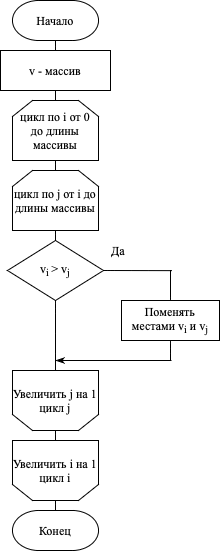
\includegraphics[scale=1]{bubble.png}
	\caption{Схема алгоритма сортировки пузырьком}
	\label{fig:bubble}
\end{figure}

\begin{figure}[h]
	\centering
	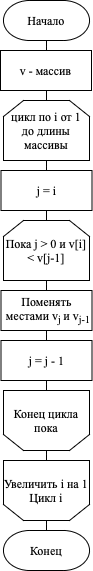
\includegraphics[scale=1]{insertion.png}
	\caption{Схема алгоритма сортировки вставками}
	\label{fig:insertion}
\end{figure}

\begin{figure}[h]
	\centering
	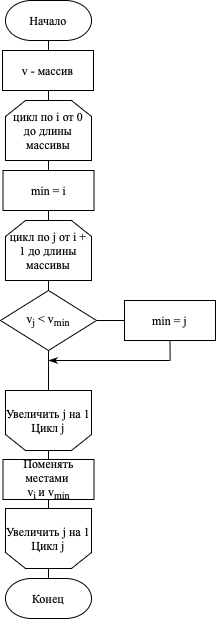
\includegraphics[scale=1]{selection.png}
	\caption{Схема алгоритма сортировки выбором}
	\label{fig:selection}
\end{figure}

\clearpage

\subsection{Вывод}

По аналитическим расчетам можно сделать вывод, что в лучшем случае быстрее всего отработает алгоритм вставками.
А в худшем случае быстрее всего отработает алгоритм пузырька.

\section{Технологическая часть}

В данном разделе будет представлен выбор языка программирования и листинги реализаций алгоритмов.

\subsection{Выбор языка программирования}
Для реализации программ я выбрал язык программирования Rust [2], так как этот язык предоставляет как низкоуровневые интерфейсы, так и высокоуровневые. Также он является безопасным языком. Среда разработки Visual Studio Code. Также данный язык был выбран потому, что в нем присутствует инструментарий для замера процессорного времени и тестирования.

\subsection{Листинги реализации алгоритма}

В листингах \ref{list:bubble} - \ref{list:selection} представлены реализации трех алгоритмов сортировки.

\begin{lstlisting}[label=list:bubble, caption=Функция сортировки массива методом пузырька]
pub fn bubble_sort<T: std::cmp::Ord>(v: &mut [T]) {
    for i in 0..v.len() {
        for j in i..v.len() {
            if v[i] > v[j] {
                v.swap(i, j);
            }
        }
    }
}
\end{lstlisting}

\begin{lstlisting}[label=list:insertion, caption=Функция сортировки массива методом вставок]
pub fn insertion_sort<T: std::cmp::Ord>(v: &mut [T]) {
    for i in 1..v.len() {
        let mut j = i;
        while j > 0 && v[j] < v[j - 1] {
            v.swap(j, j - 1);
            j = j - 1;
        }
    }
}
\end{lstlisting}

\begin{lstlisting}[label=list:selection, caption=Функция сортировки массива методом выбора]
pub fn selection_sort<T: std::cmp::Ord>(v: &mut [T]) {
    let mut min;
    for i in 0..v.len() {
        min = i;
        for j in (i + 1)..v.len() {
            if v[j] < v[min] {
                min = j;
            }
        }
        v.swap(i, min);
    }
}
\end{lstlisting}

\clearpage

\subsection{Тестирование}

Тестирование проводилось встроенной библиотекой модульного тестирования в систему сборки Cargo. \\

В таблице \ref{tab:tests} приведены результаты тестирования.

\begin{table}[h]
    \caption{\centering Результаты функционального тестирования.}
    \centering
    \begin{tabular}{|c|c|c|}
    \hline
    Вход       & Результат  & Ожидаемый результат \\ \hline
    1, 2, 3, 4 & 1, 2, 3, 4 & 1, 2, 3, 4          \\ \hline
    4, 3, 2, 1 & 1, 2, 3, 4 & 1, 2, 3, 4          \\ \hline
    1, 3, 2, 4 & 1, 2, 3, 4 & 1, 2, 3, 4          \\ \hline
    пустой     & пустой     & пустой              \\ \hline
    \end{tabular}
    \label{tab:tests}
\end{table}


\subsection*{Вывод}

В данном разделе были представлены требования к программному обеспечению, выбор языка программирования, листинги реализаций алгоритмов и результаты тестирования.

\section{Исследовательская часть}

В данном разделе будут представлены замеры времени работы реализаций алгоритмов.

\subsection{Сравнительный анализ на основе замеров времени работы алгоритмов}
	
	Был проведен замер времени работы каждого из алгоритмов с помощью библиотеки Criterion [3]. Эта библиотека замеряет процессорное время выполнения функции и усредняет его. \\

    \begin{table}[htb]
        \caption{\centering Результаты времени выполнения алгоритмов сортировок на отсортированном массиве (в секундах)}
        \centering
        \begin{tabular}{|c|c|c|c|}
        \hline
        Размер массива & Пузырек  & Вставки  & Выбором  \\ \hline
        10             & 5,50E-08 & 3,02E-08 & 6,20E-08 \\ \hline
        100            & 2,18E-06 & 1,07E-07 & 7,16E-06 \\ \hline
        500            & 4,44E-05 & 3,83E-07 & 2,24E-04 \\ \hline
        1000           & 1,69E-04 & 7,57E-07 & 9,34E-04 \\ \hline
        \end{tabular}
        \label{tab:sorted_bench}
    \end{table}

    \begin{figure}[ht]
        \centering
    \begin{tikzpicture}
        \begin{axis}[
            xlabel={Количество элементов в массиве},
            ylabel={Время (в секундах)},
            width=8cm,
            height=8cm,
            legend pos=north west,
            ymajorgrids=true,
            grid style=dashed,
        ]

        \addplot[
            color=blue,
            mark=square,
            ]
            coordinates {
                (10, 5.50e-8)(100, 2.18e-6)(500, 4.44e-5)(1000, 1.69e-4)
            };
            \addlegendentry{Пузырек}
        \addplot[
            color=red,
            mark=triangle,
            ]
            coordinates {
                (10, 3.02e-8)(100, 1.07e-7)(500, 3.82e-7)(1000, 7.57e-7)
            };
            \addlegendentry{Вставки}
        \addplot[
            color=black,
            mark=star,
            ]
            coordinates {
                (10, 6.20e-8)(100, 7.16e-6)(500, 2.24e-4)(1000, 9.34e-4)
            };
            \addlegendentry{Выбор}
    
    \end{axis}
    \end{tikzpicture}
    \caption{График времени выполнения алгоритмов при отсортированном массиве}
    \end{figure}

    \begin{table}[ht]
        \caption{\centering Результаты времени выполнения алгоритмов сортировок на отсортированном в обратном порядке массиве (в секундах)}
        \centering
        \begin{tabular}{|c|c|c|c|}
        \hline
        Размер массива & Пузырек  & Вставки  & Выбором  \\ \hline
        10             & 6,80E-08 & 8,14E-08 & 1,22E-07 \\ \hline
        100            & 2,54E-06 & 8,00E-06 & 7,55E-06 \\ \hline
        500            & 5,66E-05 & 2,01E-04 & 2,27E-04 \\ \hline
        1000           & 2,16E-04 & 8,25E-04 & 9,33E-04 \\ \hline
        \end{tabular}
        \label{tab:unsorted_bench}
    \end{table}

    \begin{figure}[ht]
    \centering
    \begin{tikzpicture}
        \begin{axis}[
            xlabel={Количество элементов в массиве},
            ylabel={Время (в секундах)},
            width=8cm,
            height=8cm,
            legend pos=north west,
            ymajorgrids=true,
            grid style=dashed,
        ]

        \addplot[
            color=blue,
            mark=square,
            ]
            coordinates {
                (10, 6.80e-08)(100, 2.54e-06)(500, 5.66e-05)(1000, 2.16e-04)
            };
            \addlegendentry{Пузырек}
        \addplot[
            color=red,
            mark=triangle,
            ]
            coordinates {
                (10, 8.14e-08)(100, 8.00e-06)(500, 2.01e-04)(1000, 8.25e-04)
            };
            \addlegendentry{Вставки}
        \addplot[
            color=black,
            mark=star,
            ]
            coordinates {
                (10, 1.22e-07)(100, 7.55e-06)(500, 2.27e-04)(1000, 9.33e-04)
            };
            \addlegendentry{Выбор}
    
    \end{axis}
    \end{tikzpicture}
    \caption{График времени выполнения алгоритмов при отсортированном в обратном порядке массиве}
    \end{figure}

    \begin{table}[ht]
        \caption{\centering Результаты времени выполнения алгоритмов сортировок на случайном массиве (в секундах)}
        \centering
        \begin{tabular}{|c|c|c|c|}
        \hline
        Размер массива & Пузырек  & Вставки  & Выбором  \\ \hline
        100            & 2,91E-06 & 3,75E-06 & 8,72E-06 \\ \hline
        1000           & 3,32E-04 & 4,11E-04 & 9,48E-04 \\ \hline
        2500           & 2,02E-03 & 2,55E-03 & 5,99E-03 \\ \hline
        5000           & 8,27E-03 & 1,02E-02 & 2,43E-02 \\ \hline
        \end{tabular}
        \label{tab:rand_bench}
    \end{table}

    \begin{figure}[ht]
        \centering
    \begin{tikzpicture}
        \begin{axis}[
            xlabel={Количество элементов в массиве},
            ylabel={Время (в секундах)},
            width=10cm,
            height=8cm,
            legend pos=north west,
            ymajorgrids=true,
            grid style=dashed,
        ]

        \addplot[
            color=blue,
            mark=square,
            ]
            coordinates {
                (100, 2.91e-06)(1000, 3.32e-04)(2500, 2.02e-03)(5000, 8.27e-03)
            };
            \addlegendentry{Пузырек}
        \addplot[
            color=red,
            mark=triangle,
            ]
            coordinates {
                (100, 3.75e-06)(1000, 4.11e-04)(2500, 2.55e-03)(5000, 1.02e-02)
            };
            \addlegendentry{Вставки}
        \addplot[
            color=black,
            mark=star,
            ]
            coordinates {
                (100, 8.72e-06)(1000, 9.48e-04)(2500, 5.99e-03)(5000, 2.43e-02)
            };
            \addlegendentry{Выбор}
    
    \end{axis}
    \end{tikzpicture}
    \caption{График времени выполнения алгоритмов при случайном массиве}
    \end{figure}

    \clearpage

    \subsection*{Вывод}

    По результатам тестирования выявлено, что все рассматриваемые алгоритмы реализованы правильно. Самым быстрым алгоритмом при использовании случайного массива оказался алгоритм сортировки методом пузырька. Метод выбора является самый медленным на случайном наборе данных. Теоретические данные совпали с экспериментальными.

    \anonsection{Заключение}

    В рамках данной лабораторной работы была достигнута цель и выполнены следующие задачи:

    \begin{itemize}
        \item были изучены и реализованы три алгоритма сортировки: методом пузырька, вставок и выбором;
        \item был проведен сравнительный анализ трудоемкости алгоритмов на основе теоретических расчетов и выбранной модели вычислений;
        \item был проведен сравнительный анализ алгоритмов на основе экспериментальных данных.
    \end{itemize}

    Экспериментально были установлены различия в производительности различных алгоритмов сортировки. Для массивов длины 5000, заполненной случайными данными, метод пузырька быстрее вставок и выбора.

    \anonsection{Литература}

    \begin{enumerate}
    \item Блэнди Дж., Орендорф Дж. Программирование на языке Rust = Programming Rust. — ДМК Пресс, 2018. — 550 с. — ISBN 978-5-97060-236-2.
    \item Criterion.rs - Statistics-driven benchmarking library for Rust [Электронный ресурс] \url{https://github.com/bheisler/criterion.rs} (дата обращения: \today)
    \item LPDDR4 [Электронный ресурс] \url{https://ru.wikipedia.org/wiki/LPDDR#LPDDR4} (дата обращения: \today)
\end{enumerate}


\end{document}
